% Options for packages loaded elsewhere
\PassOptionsToPackage{unicode,citecolor=black}{hyperref}
\PassOptionsToPackage{hyphens}{url}
\PassOptionsToPackage{dvipsnames,svgnames,x11names}{xcolor}
%
\documentclass[
  authoryear,
  3p]{elsarticle}

\usepackage{amsmath,amssymb}
\usepackage{iftex}
\ifPDFTeX
  \usepackage[T1]{fontenc}
  \usepackage[utf8]{inputenc}
  \usepackage{textcomp} % provide euro and other symbols
\else % if luatex or xetex
  \usepackage{unicode-math}
  \defaultfontfeatures{Scale=MatchLowercase}
  \defaultfontfeatures[\rmfamily]{Ligatures=TeX,Scale=1}
\fi
\usepackage{lmodern}
\ifPDFTeX\else  
    % xetex/luatex font selection
\fi
% Use upquote if available, for straight quotes in verbatim environments
\IfFileExists{upquote.sty}{\usepackage{upquote}}{}
\IfFileExists{microtype.sty}{% use microtype if available
  \usepackage[]{microtype}
  \UseMicrotypeSet[protrusion]{basicmath} % disable protrusion for tt fonts
}{}
\makeatletter
\@ifundefined{KOMAClassName}{% if non-KOMA class
  \IfFileExists{parskip.sty}{%
    \usepackage{parskip}
  }{% else
    \setlength{\parindent}{0pt}
    \setlength{\parskip}{6pt plus 2pt minus 1pt}}
}{% if KOMA class
  \KOMAoptions{parskip=half}}
\makeatother
\usepackage{xcolor}
\setlength{\emergencystretch}{3em} % prevent overfull lines
\setcounter{secnumdepth}{5}
% Make \paragraph and \subparagraph free-standing
\makeatletter
\ifx\paragraph\undefined\else
  \let\oldparagraph\paragraph
  \renewcommand{\paragraph}{
    \@ifstar
      \xxxParagraphStar
      \xxxParagraphNoStar
  }
  \newcommand{\xxxParagraphStar}[1]{\oldparagraph*{#1}\mbox{}}
  \newcommand{\xxxParagraphNoStar}[1]{\oldparagraph{#1}\mbox{}}
\fi
\ifx\subparagraph\undefined\else
  \let\oldsubparagraph\subparagraph
  \renewcommand{\subparagraph}{
    \@ifstar
      \xxxSubParagraphStar
      \xxxSubParagraphNoStar
  }
  \newcommand{\xxxSubParagraphStar}[1]{\oldsubparagraph*{#1}\mbox{}}
  \newcommand{\xxxSubParagraphNoStar}[1]{\oldsubparagraph{#1}\mbox{}}
\fi
\makeatother


\providecommand{\tightlist}{%
  \setlength{\itemsep}{0pt}\setlength{\parskip}{0pt}}\usepackage{longtable,booktabs,array}
\usepackage{calc} % for calculating minipage widths
% Correct order of tables after \paragraph or \subparagraph
\usepackage{etoolbox}
\makeatletter
\patchcmd\longtable{\par}{\if@noskipsec\mbox{}\fi\par}{}{}
\makeatother
% Allow footnotes in longtable head/foot
\IfFileExists{footnotehyper.sty}{\usepackage{footnotehyper}}{\usepackage{footnote}}
\makesavenoteenv{longtable}
\usepackage{graphicx}
\makeatletter
\def\maxwidth{\ifdim\Gin@nat@width>\linewidth\linewidth\else\Gin@nat@width\fi}
\def\maxheight{\ifdim\Gin@nat@height>\textheight\textheight\else\Gin@nat@height\fi}
\makeatother
% Scale images if necessary, so that they will not overflow the page
% margins by default, and it is still possible to overwrite the defaults
% using explicit options in \includegraphics[width, height, ...]{}
\setkeys{Gin}{width=\maxwidth,height=\maxheight,keepaspectratio}
% Set default figure placement to htbp
\makeatletter
\def\fps@figure{htbp}
\makeatother

\usepackage{fvextra}
\DefineVerbatimEnvironment{Highlighting}{Verbatim}{breaklines,commandchars=\\\{\}}
\makeatletter
\@ifpackageloaded{caption}{}{\usepackage{caption}}
\AtBeginDocument{%
\ifdefined\contentsname
  \renewcommand*\contentsname{Table of contents}
\else
  \newcommand\contentsname{Table of contents}
\fi
\ifdefined\listfigurename
  \renewcommand*\listfigurename{List of Figures}
\else
  \newcommand\listfigurename{List of Figures}
\fi
\ifdefined\listtablename
  \renewcommand*\listtablename{List of Tables}
\else
  \newcommand\listtablename{List of Tables}
\fi
\ifdefined\figurename
  \renewcommand*\figurename{Figure}
\else
  \newcommand\figurename{Figure}
\fi
\ifdefined\tablename
  \renewcommand*\tablename{Table}
\else
  \newcommand\tablename{Table}
\fi
}
\@ifpackageloaded{float}{}{\usepackage{float}}
\floatstyle{ruled}
\@ifundefined{c@chapter}{\newfloat{codelisting}{h}{lop}}{\newfloat{codelisting}{h}{lop}[chapter]}
\floatname{codelisting}{Listing}
\newcommand*\listoflistings{\listof{codelisting}{List of Listings}}
\makeatother
\makeatletter
\makeatother
\makeatletter
\@ifpackageloaded{caption}{}{\usepackage{caption}}
\@ifpackageloaded{subcaption}{}{\usepackage{subcaption}}
\makeatother
\journal{Journal of the Acoustical Society of America}

\ifLuaTeX
  \usepackage{selnolig}  % disable illegal ligatures
\fi
\usepackage[]{natbib}
\bibliographystyle{elsarticle-harv}
\usepackage{bookmark}

\IfFileExists{xurl.sty}{\usepackage{xurl}}{} % add URL line breaks if available
\urlstyle{same} % disable monospaced font for URLs
\hypersetup{
  pdftitle={Soundscape Perception Indices (SPI): Developing context-dependent single value scores of multidimensional soundscape perceptual quality},
  pdfauthor={Andrew Mitchell; Francesco Aletta; Tin Oberman; Jian Kang},
  pdfkeywords={Soundscape, Sound perception, index, urban design},
  colorlinks=true,
  linkcolor={blue},
  filecolor={Maroon},
  citecolor={Blue},
  urlcolor={Blue},
  pdfcreator={LaTeX via pandoc}}


\setlength{\parindent}{6pt}
\begin{document}

\begin{frontmatter}
\title{Soundscape Perception Indices (SPI): Developing context-dependent
single value scores of multidimensional soundscape perceptual quality}
\author[1,2]{Andrew Mitchell%
\corref{cor1}%
}
 \ead{a.j.mitchell@ucl.ac.uk} 
\author[2]{Francesco Aletta%
%
}
 \ead{f.aletta@ucl.ac.uk} 
\author[2]{Tin Oberman%
%
}
 \ead{t.oberman@ucl.ac.uk} 
\author[2]{Jian Kang%
%
}
 \ead{j.kang@ucl.ac.uk} 

\affiliation[1]{organization={University College London, Bartlett School
of Sustainable Construction},addressline={1-19 Torrington
Place},city={London},postcodesep={}}
\affiliation[2]{organization={University College London, Institute for
Environmental Design and Engineering},addressline={Central House, 14
Upper Woburn Place},city={London},postcode={WC1H 0NN},postcodesep={}}

\cortext[cor1]{Corresponding author}




        
\begin{abstract}
The soundscape approach provides a basis for considering the holistic
perception of sound environments, in context. While steady advancements
have been made in methods for assessment and analysis, a gap exists for
comparing soundscapes and quantifying improvements in the
multi-dimensional perception of a soundscape. To this end, there is a
need for the creation of single value indices to compare soundscape
quality which incorporate context, aural diversity, and specific design
goals for a given application. Just as a variety of decibel-based
indices have been developed for various purposes (e.g.~\(L_{Aeq}\),
\(L_{Ceq}\), \(L_{90}\), \(L_{den}\), etc.), the soundscape approach
requires the ability to create novel indices for different uses, which
share a common language and understanding. We therefore propose a
unified framework for creating bespoke and reference single index
measures of soundscape perception, allowing for new metrics to be
defined in the future. This framework is based on a four-step
test-target paradigm wherein a desired soundscape perception is defined
as a target distribution within the soundscape circumplex and the 2D
Kolmogorov-Smirnov distance is used to test an assessed soundscape
against this target. Applications and implications of this framework are
discussed and a multi-objective optimisation method for empirically
defining perception indices is proposed.
\end{abstract}





\begin{keyword}
    Soundscape \sep Sound perception \sep index \sep 
    urban design
\end{keyword}
\end{frontmatter}
    
\RecustomVerbatimEnvironment{verbatim}{Verbatim}{
  showspaces = false,
  showtabs = false,
  breaksymbolleft={},
  breaklines
  % Note: setting commandchars=\\\{\} here will cause an error 
  }


\section{Introduction}\label{sec-introduction}

The EU Green Paper on Future Noise Policy indicates that 80 million EU
citizens are suffering from potentially harmful environmental noise
levels, according to the World Health Organization (WHO) recommendations
\citep{Berglund1999Guidelines}. The publication of the EU Directive
Relating to the Assessment and Management of Environmental Noise (END)
\citep{EuropeanUnion2002Directive} more than two decades ago has led to
major actions across Europe, with reducing noise levels as their main
focus, for which billions of Euros are being spent. However, it is
widely recognised that solely reducing sound level in people's living
environments is not always feasible or cost-effective and, more
importantly, with only \textasciitilde30\% of environmental noise
annoyance depending on physical aspects of the signal such as acoustic
energy \citep{Guski1997Psychological}, sound level reduction will not
necessarily lead to improved quality of life. For this reason, from a
public health point of view, it is necessary to explore alternative
management and design strategies for acoustic environments that rely on
more positive soundscapes, rather than merely environments not affected
by noise pollution
\citep{Aletta2018Associations, Kang2023Soundscape, Kang2023Supportive}.

Soundscape design, separate from (and complementary to) noise control
engineering, is about the relationships between human physiology,
perception, the sound environment, and its socio-cultural context
\citep{Kang2006Urban}. Soundscape research represents a paradigm shift
in that it combines physical, social, and psychological approaches and
considers environmental sounds as a `resource' rather than `waste'
\citep{Kang2016Soundscape} relating to perceptual constructs rather than
just physical phenomena. However, the current research is still at the
stage of describing and identifying the problems and tends to be
fragmented and focussed on only special cases
e.g.\textasciitilde subjective evaluations of soundscapes for
residential areas
\citep{SchulteFortkamp2013Introduction, Chen2023Natural}. In the
movement from noise control to soundscape creation
\citep{Aletta2015Soundscape}, a vital step is the standardisation of
methods to assess soundscape quality.

A common aim for implementing soundscape assessment in practice is to
compare the quality of different soundscapes. Often (but not always) the
goal is to identify a `good' soundscape compared to a `bad' soundscape.
However, this presents several challenges:

\begin{itemize}
\tightlist
\item
  What makes a soundscape good or bad is highly contextual; that is, the
  same acoustic environment may result in different appreciations and
  perceptual outcomes, depending on where/when it is happening, and what
  groups of individuals are there to experience it.
\item
  On what metric should the quality rating be based? Previous attempts
  at defining objective metrics of ``soundscape quality'' assessment
  have fallen short of capturing the multidimensionality of people's
  perception of surrounding acoustic environments.
\item
  How can we deal with different requirements and definitions of how a
  soundscape should be perceived? Soundscape constructs are normally
  seen as highly individualised, while designing the soundscapes of
  public spaces should look at accommodating the needs of a given
  community of a space as a whole.
\end{itemize}

In many cases, the ultimate aim is to be able to rank soundscapes based
on their quality. There is pressure from stakeholders and policymakers
to move towards such simplified assessment protocols. However, any
ranking metric should be flexible and be able to handle a variety of
contexts and definitions of what a `good' soundscape is for a given
purpose. To address this, we will propose the Soundscape Perception
Index (SPI) framework, a flexible method for defining single value
indices of soundscape quality based on distributions within the
Soundscape Circumplex Model (SCM)
\citep{Axelsson2012Swedish, Mitchell2022How, Axelsson2010principal}. As
previously suggested, the primary motivation behind the development of
the Soundscape Perception Indices (SPI) framework stems from the need to
address the existing gap in quantifying and comparing soundscape quality
across diverse contexts and applications. By creating a unified
framework for defining these indices, the aim is to is to empower
stakeholders, decision-makers, and researchers with the ability to
create tailored indices that align with their specific objectives and
design goals, while simultaneously enabling cross-comparisons and
benchmarking against empirically-defined reference soundscapes. This
dual approach not only acknowledges the context-dependent nature of
soundscape perception but also fosters a common language and
understanding, facilitating knowledge sharing and collaborative efforts
within the field. This paper will demonstrate the SPI framework and test
whether it is capable of both scoring soundscape quality and generating
consistent rankings of soundscapes across different contexts.

\section{Theoretical Background}\label{sec-theoretical-background}

In \citet{Aletta2016Soundscape}, the authors defined a framework for
categorising the components of a soundscape assessment. They define
three aspects: soundscape descriptors, soundscape indicators, and
soundscape indices. Soundscape descriptors are defined as `measures of
how people perceive the acoustic environment' and soundscape indicators
as `measures used to predict the value of a soundscape descriptor'. The
relationship between soundscape indicator(s) and a soundscape descriptor
effectively defines what has been previously referred to as a
``predictive soundscape model''
\citep{Aletta2016Soundscape, Mitchell2022Predictive}. There are
primarily two rationales for modeling the relationship between the
physical attributes and the perceived (i.e., soundscape) qualities of
the acoustic environment. Firstly, a predictive model can forecast how
individuals would perceive the acoustic environment, eliminating the
need for labour-intensive surveys \citep{Mitchell2023conceptual}.
Secondly, a precise predictive model may unveil the root causes of these
perceived qualities, thereby serving as a valuable tool for design.
\citet{Lionello2020systematic} provided a review of such models and
concluded contextual features play an important role in increasing the
quality of the model. Indices on the other hand, the primary focus of
this article, are single numerical values that combine multiple
indicators or descriptors to provide a comprehensive representation of
the overall soundscape perception and allow for comparison between
soundscapes.

The earliest and most commonly used scientific index measuring sound
level is the Decibel (dB). To represent the overall level of sound with
a single value on one scale, as the Decibel index does, is often
desirable. For this purpose, a number of different values representing
sounds at various frequencies must be combined. Several frequency
weighting networks have been developed since the 1930s, considering
typical human responses to sound based on equal-loudness-level contours
\citep{Fletcher1933Loudness} and, among them, the A-weighting network,
with resultant decibel values called dBA, has been commonly used in
almost all the national/international regulations
\citep{Kryter1994Handbook}. However, there have been numerous criticisms
on its effectiveness \citep{Parmanen2007weighted} as the correlations
between dBA and perceived sound quality (e.g.\textasciitilde noise
annoyance) are often low \citep{Hellman1987Why}.

Another set of indices is psychoacoustic magnitudes, including loudness,
fluctuation strength or roughness, sharpness, and pitch strength,
developed through sound quality studies of industrial products since the
1980's \citep{Zwicker2007Psychoacoustics}. These emerged when it was
conceived that acoustic emissions can be characterised beyond just sound
level \citep{Blauert1997Sound}. But while psychoacoustic magnitudes have
proven to be successful for the assessment of product sound quality, in
the field of environmental acoustics, their applicability has been
limited \citep{Fastl2006Psychoacoustic}, since a significant feature of
environmental acoustics is that there are multiple/dynamic sound
sources. Additionally, while pyschoacoustic magnitudes incorporate
perceptual aspects, both dB based and pyschoacoustic indicies are
ultimately describing the acoustic signal and not the soundscape
perception and may therefore be more accurately described as indicators
rather than soundscape indices \citep{Mitchell2023conceptual}.

When applied to urban sound and specifically to noise pollution, the
soundscape approach introduces three key considerations beyond
traditional noise control methods:

\begin{enumerate}
\def\labelenumi{\arabic{enumi}.}
\tightlist
\item
  considering all aspects of the environment which may influence
  perception, not just the sound level and spectral content (e.g.,
  visual setting, odour environment, spatial layout, etc.);
\item
  an increased and integrated consideration of the varying impacts which
  different sound sources and sonic characteristics have on perception;
  and
\item
  a consideration of both the positive and negative dimensions of
  soundscape perception.
\end{enumerate}

This approach can enable better outcomes by identifying positive
soundscapes (in line with the END's mandate to ``preserve environmental
noise quality where it is good'' \citep{EuropeanUnion2002Directive}),
better identifying specific sources of noise which impact soundscape
quality and pinpointing the characteristics which may need to be
decreased, and illuminating alternative methods which could be
introduced to improve a soundscape where a reduction of noise is
impractical \citep{Fiebig2018Does, Kang2018Impact}. Factors such as the
presence of natural or human-made sounds, their temporal patterns, and
the overall contextual meaning ascribed to these sounds all contribute
to the holistic perception of a soundscape.

\subsection{Existing `Soundscape
Indices'}\label{sec-existing-soundscape-indices}

While the field of soundscape research has witnessed substantial
progress, the development of standardized indices for evaluating and
comparing soundscapes across diverse contexts has been relatively
limited. Existing indices can be broadly seen as arising from two
domains: soundscape ecology and soundscape perception.

\subsubsection{Soundscape Ecology and
Bioacoustics}\label{sec-soundscape-ecology-and-bioacoustics}

Within the realm of soundscape ecology, indices such as the Acoustic
Diversity Index (ADI) and Frequency-dependent Acoustic Diversity Index
(FADI) \citep{Xu2023frequency} have been developed to quantify the
diversity and complexity of acoustic signals within a given soundscape.
Similar indices (e.g.~ADI, NDSI, ACI) have also been developed to
analyse the acoustic signal of complex acoustic environments and
indicate the richness and diversity of biophonic (natural) and
anthrophonic (human-made) sound sources. However, while these indices
contribute valuable insights into the ecological aspects of soundscapes,
they do not directly address the perceptual dimensions that are central
to the soundscape approach \citep{SchulteFortkamp2023Soundscapes}. The
multi-dimensional nature of soundscape perception, encompassing factors
such as pleasantness, eventfulness, and familiarity, necessitates a more
comprehensive and context-sensitive approach.

\subsubsection{Soundscape Perception}\label{sec-soundscape-perception}

In the domain of soundscape perception, several indices have emerged as
attempts to quantify the perceived quality of soundscapes, particularly
in urban environments.

The Green Soundscape Index (GSI) \citep{Kogan2018Green} incorporates
factors such as the presence and levels of natural sounds and human-made
sounds, and their respective contributions to the overall soundscape
perception. The GSI is defined as the ratio of the perceived extent of
natural sounds (PNS) to the perceived extent of traffic noise (PTN),
ranging between 1/5 and 5. Subsequently, Cao and colleagues
\citep{Cao2020Red, Yang2022Effects} proposed the Red Soundscape Index
(\(RSI\)), defined as the ratio of the perceived extent of human sounds
to the perceived extent of either natural sounds (\(RSI_n\)) or traffic
sounds (\(RSI_t\)), arguing that the GSI alone was not suitable for all
urban soundscape design applications.

Building on ecological diversity concepts, \citet{Liu2014Effects}
introduced the Soundscape Diversity Index (SDI), which quantifies the
probability of two randomly selected sounds in a soundscape belonging to
different categories, providing a measure of soundscape complexity.
Expanding on this approach, \citet{Xiang2023Soundscape} defined an
expanded set of soundscape diversity indices, including the SDI, the
Soundscape Richness Index (SRI), the Soundscape Dominance Index (SDO),
and the Soundscape Evenness Index (SEI). These indices, adapted from
species diversity measures in ecology, offer a more nuanced approach to
quantifying aspects of soundscape perception.
\citet{Xiang2023Soundscape} demonstrated that these indices could be
partially explained by existing acoustic indicators and were more
suitable for evaluating urban green spaces than traditional acoustic
indices.

\citet{Guo2023Harmonious} proposed the Harmonious Degree of Sound
Sources (SHD) index, which combines perceived loudness, occurrence, and
preference for sound sources. The SHD assess how well the dominance of a
sound aligns with visitors' preferences, aiming to reflect the
harmonious status of sounds in a soundscape.

In 2019, \citet{Kang2019Towards} proposed the development of a set of
soundscape indices (SSID) which might take the form
\(SSID = f(\text{physical factors}) + f(\text{contextual factors}) + \ldots\)
where the functions and weights of each aspect influencing soundscape
perception (i.e.~physical/acoustic parameters, contextual and visual
factors, personal factors, etc.) could be derived statistically from a
large dataset of soundscape surveys. The work presented here represents
a development of this thinking which has grown out of the SSID project,
where the analysis and indexing of perception data and the connection
between soundscape indicators and perception have been separated
\citep{Mitchell2023conceptual}. This modularization of perception
prediction based on objective factors and soundscape index creation
should enable more sophisticated and thoughtful index creation and more
advanced and updateable prediction models.

While these indices offer valuable insights into specific aspects of
soundscape perception, they are limited in their ability to capture the
full multidimensionality of soundscape experienve across diverse
contexts. The Soundscape Perception Index (SPI) framework presented in
this paper builds upon these efforts by providing a flexible,
context-sensitive approach to soundscape assessment. Unlike many
previous indices, the SPI is not an analysis of an acoustic signal but
rather is an index of perception based on soundscape descriptors.
Furthermore, it does not represent a single target in a particular
context, but is a generalisable, extensible, and adaptable framework for
scoring soundscapes against any goal defined by the user.

The remainder of the paper will introduce and demonstrate this
framework, providing a case study of defining an appropriate target.

\section{Establishing the SPI Framework}\label{sec-method}

The index framework, `Soundscape Perception Indices (SPI)' introduced in
this paper is defined here as the agreement between an observed or
modelled soundscape perception distribution and a target soundscape
perception distribution. Its goal is to determine whether a soundscape -
whether it be a real-world location, a proposed design, or a
hypothetical scenario - aligns with the desired (or reference)
perception of that soundscape. This is achieved by first defining the
target distribution, which could represent what is considered to be the
`ideal' soundscape perception for a given context or application. The
test distribution is then compared to the target distribution using a
distance metric, which quantifies the deviation between the two
distributions. The resulting distance value serves as the basis for
calculating the SPI, with smaller distances indicating a closer
alignment between the perceived soundscape and the target soundscape
perception.

We refer to this as an index framework rather than a single index, as
the SPI can be tailored to specific contexts and applications by
defining a range of target distributions. A single index is thus created
for each target distribution. An SPI value therefore does not represent
a `good' or `bad' soundscape, but rather a measure of how closely the
perceived soundscape aligns with the desired target soundscape
perception. This approach allows for the development of bespoke indices
tailored to specific design goals and objectives, while also enabling
cross-comparisons and benchmarking against empirically-defined reference
soundscape targets.

\subsection{Core Method}\label{sec-core-method}

SPI is grounded in the soundscape circumplex model (SCM)
\citep{Axelsson2010principal, Axelsson2012Swedish}, a robust theoretical
foundation for understanding and representing the multi-dimensional
nature of soundscape perception. The reason for grounding the SPI in the
soundscape circumplex is that we have observed this model to become the
most prevalent assessment model in soundscape literature
\citep{Aletta2023Adoption}. The SCM is built on a series of descriptors
referred to as the Perceived Affective Quality (PAQ), proposed by
\citep{Axelsson2010principal}. These PAQs are based on the
pleasantness-eventfulness paradigm adopted in research on emotions and
environmental psychology (and its original version, conceptualized as
valence-arousal paradigm), in particular Russell's circumplex model of
affect \citep{Russell1980circumplex}. As summarised by
\citet{Axelsson2010principal}: ``Russell's model identifies two
dimensions related to the perceived pleasantness of environments and how
activating or arousing the environment is.''

One benefit of the circumplex model is that, as a whole, it encapsulates
several of the other proposed soundscape descriptors - in particular,
annoyance, pleasantness, tranquillity, and possibly restorativeness
\citep{Aletta2016Soundscape}. According to \citet{Axelsson2015How}, the
two-dimensional circumplex model of perceived affective quality provides
the most comprehensive information for soundscape assessment. It is also
possible that the overall soundscape quality could itself be derived
from the pleasant-eventful scores derived for a soundscape. The
circumplex also lends itself well to questionnaire-based methods of data
collection, as proposed in \citet{ISO12913Part2}. In contrast to methods
such as soundwalks, interviews, and lab experiments, \emph{in situ}
questionnaires are able to provide the quality and amount of data which
is necessary for statistical modelling. Combined, these factors make the
circumplex most appropriate for a single index as it provides a
comprehensive summary of soundscape perception.

There are four steps involved in calculating the SPI, as shown in
Figure~\ref{fig-bespoke-spi}:

\begin{enumerate}
\def\labelenumi{\arabic{enumi}.}
\tightlist
\item
  Define and parameterise the target circumplex distribution;
\item
  Sample the target distribution and prepare the test distribution;
\item
  Compare test and target distributions using the distance metric
  (two-dimensional Kolmogorov-Smirnov distance \(D_{BKS}\));
\item
  Calculate \(SPI = 100 * (1 - D_{BKS})\).
\end{enumerate}

\begin{figure*}

\centering{

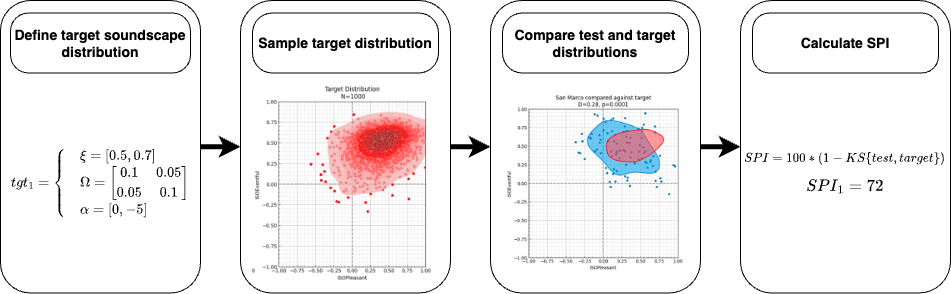
\includegraphics[width=1\textwidth,height=\textheight]{figures/SPI-framework.drawio.png}

}

\caption{\label{fig-bespoke-spi}Steps for calculating the SPI.}

\end{figure*}%

These steps and their required background are discussed in detail in the
following sections. Section~\ref{sec-targets} will then present
strategies for defining targets and their applications. Throughout this
paper, we use the data contained in the International Soundscape
Database (ISD) \citep{Mitchell2024International}, which includes 1300+
individual responses on the PAQ scales collected across 13 locations in
London and Venice, according to the SSID Protocol
\citep{Mitchell2020Soundscape}.

\subsection{Define and Parameterise a Soundscape Circumplex
Distribution}\label{sec-circumplex-distribution}

To move the eight-item PAQ responses into the two-dimensional circumplex
space, we use the projection method first presented in ISO/TS
12913-3:2018 \citep{ISO12913Part3}. This projection method and its
associated formulae were recently updated further in
\citet{Aletta2024Soundscape} to include a correction for the language in
which the survey was conducted. \citet{Aletta2024Soundscape} also
provides adjusted angles for translations of the circumplex attributes
to be used in calculating the \(P_{ISO}\) and \(E_{ISO}\) coordinates.
Once the individual perceptual responses are projected into the
circumplex space, the resulting data for each location is treated as a
circumplex distribution. There are several advancements in considering
circumplex distributions compared to the discussions originally given in
\citet{Mitchell2022How} which are necessary for SPI. Before exploring
the SPI method and target setting more specifically, we will first
address these developments.

The circumplex is defined by two axes: \(P_{ISO}\) and \(E_{ISO}\),
which are limited to the range \([-1, +1]\). Typically, data in the
soundscape circumplex is treated as a combination of two independent
normal distributions, one for each axis
\citep{Mitchell2022How, Ooi2022Probably}. In some applications this
approach is sufficient for capturing the distribution of soundscape
perception, however defining a target distribution for SPI requires a
more precise approach. The independent normal distribution approach
relies on three key assumptions:

\begin{enumerate}
\def\labelenumi{\arabic{enumi}.}
\tightlist
\item
  The two axes are normally distributed.
\item
  The two axes are symmetrically distributed.
\item
  The two axes are independent of each other.
\end{enumerate}

While the first assumption is generally valid, the second and third
assumptions are not always met in practice. In particular, the
distribution of soundscape perception responses in the circumplex is
often characterised by a high degree of skewness, which can lead to
inaccuracies in the calculation of the SPI. Soundscape circumplex
distributions are most appropriately described as a bivariate
skew-normal distribution \citep{Azzalini2005Skew} which accurately
reflects the relationship between the two dimensions of the circumplex
and the fact that real-world perceptual distributions have been
consistently observed to not be strictly symmetric.

The skew-normal distribution is defined by three parameters: location
(\(\mu\)), scale (\(\sigma\)), and shape (\(\alpha\)). The location
parameter defines the centre of the distribution, the scale parameter
defines the spread of the distribution and the shape parameter defines
the skew of the distribution. The one-dimensional skew-normal
distribution is defined as \citep{Azzalini1996Multivariate}:

\[
\phi(z; \alpha) = 2 \phi(z) \Phi(\alpha z) \quad \text{for} \quad z \in \mathbb{R}
\]

where \(\phi\) and \(\Phi\) are the standard normal probability density
function and distribution function, respectively, and \(\alpha\) is a
shape variable which regulates the skewness. The distribution reduces to
a standard normal density when \(\alpha = 0\). The bivariate skew-normal
distribution extends this concept to two dimensions, allowing for the
modelling of asymmetric and skewed distributions in a two-dimensional
space such as the soundscape circumplex. The multivariate skew-normal
(MSN) distribution including scale and location parameters is given by
combining the normal density and distribution functions
\citep{Azzalini1999Statistical}:

\[
Y = 2 \phi_k (y-\xi; \Omega) \Phi\{\alpha^T\omega^{-1}(y-\xi)\}
\]

where \(\phi_k\) is the \emph{k}-dimensional normal density with
location \(\xi\), shape \(\alpha\), and covariance matrix \(\Omega\).
\(\Phi \{ \dot \}\) is the normal distribution function and \(\alpha\)
is a \emph{k}-dimensional shape vector. When \(\alpha = 0\), \(Y\)
reduces to the standard multivariate normal \(N_k(\xi, \Omega)\)
density. A circumplex distribution can therefore be
parameterised\footnote{It is important to note that the parameters which
  appear in the density expression (\(\xi, \Omega, \alpha\)) are what
  are called `direct parameters' (DP). They directly parameterise an MSN
  density and are typically only estimated by fitting an MSN to a
  sample. The more familiar and interpretable components (mean, standard
  deviation, and skewness) are termed the centred parameters (CP). It is
  possible to move from one parameterization to another, however ``while
  any choice of the DP components is admissible, the same is not true
  for CP''; i.e.~we can always move DP \(\rightarrow\) CP but not always
  CP \(\rightarrow\) DP. In this context, it is most important for
  readers not to confuse the location parameter \(\xi\) with the sample
  mean \(\mu\). A more complete explanation of these parameterizations
  can be found in \citet{Azzalini2016How}} with a 2x2 covariance matrix
\(\Omega\), a 2x1 location vector \(\xi\), and a 2x1 shape vector
\(\alpha\), written as:

\[
Y \sim MSN (\xi, \Omega, \alpha)
\]

By fitting an MSN distribution to empirical soundscape perception
responses, it becomes possible to accurately capture the asymmetry and
skewness of the distribution. A bivariate skew-normal distribution can
be summarised as a set of these three parameters. Once parameterised,
the distribution can then be sampled from to generate a synthetic
distribution of soundscape perception responses.

Soundscape targets can thus be set by defining the desired MSN
distribution. To demonstrate this, we will construct three arbitrary
targets which will be used later to score three SPIs. The parameters
chosen for the example targets are given in
Table~\ref{tbl-target-params}.

\begin{longtable}[]{@{}
  >{\centering\arraybackslash}p{(\columnwidth - 6\tabcolsep) * \real{0.1455}}
  >{\centering\arraybackslash}p{(\columnwidth - 6\tabcolsep) * \real{0.1455}}
  >{\centering\arraybackslash}p{(\columnwidth - 6\tabcolsep) * \real{0.5636}}
  >{\centering\arraybackslash}p{(\columnwidth - 6\tabcolsep) * \real{0.1455}}@{}}
\caption{The MSN direct parameterizations for three arbitrary example
target distributions. \(\text{tgt}_1\) is located in the pleasant half,
with a wide variance, and a positive skew along the pleasantness axis.
\(\text{tgt}_2\) is located in the calm quadrant, with a typical
variance, and a negative skew along the pleasantness axis and a positive
skew along the eventful axis. \(\text{tgt}_3\) is located in the vibrant
quadrant, with a moderate variance, and a negative skew along the
eventfulness axis.}\label{tbl-target-params}\tabularnewline
\toprule\noalign{}
\begin{minipage}[b]{\linewidth}\centering
Target
\end{minipage} & \begin{minipage}[b]{\linewidth}\centering
Location \(\xi\)
\end{minipage} & \begin{minipage}[b]{\linewidth}\centering
Covariance Matrix \(\Omega\)
\end{minipage} & \begin{minipage}[b]{\linewidth}\centering
Shape \(\alpha\)
\end{minipage} \\
\midrule\noalign{}
\endfirsthead
\toprule\noalign{}
\begin{minipage}[b]{\linewidth}\centering
Target
\end{minipage} & \begin{minipage}[b]{\linewidth}\centering
Location \(\xi\)
\end{minipage} & \begin{minipage}[b]{\linewidth}\centering
Covariance Matrix \(\Omega\)
\end{minipage} & \begin{minipage}[b]{\linewidth}\centering
Shape \(\alpha\)
\end{minipage} \\
\midrule\noalign{}
\endhead
\bottomrule\noalign{}
\endlastfoot
\(\text{tgt}_1\) & \([0.5, 0.0]\) &
\(\begin{bmatrix} 0.2 & 0.0 \\ 0.0 & 0.2 \end{bmatrix}\) & \([1, 0]\) \\
\(\text{tgt}_2\) & \([1.0, -0.4]\) &
\(\begin{bmatrix} 0.18 & -0.04 \\ -0.04 & 0.09 \end{bmatrix}\) &
\([-8, 1]\) \\
\(\text{tgt}_3\) & \([0.5, 0.7]\) &
\(\begin{bmatrix} 0.1 & 0.05 \\ 0.05 & 0.1 \end{bmatrix}\) &
\([0, -5]\) \\
\end{longtable}

\subsection{Sample a Target
Distribution}\label{sec-sample-a-target-distribution}

Once the parameters for an MSN are defined (i.e., the target), the MSN
is then sampled using the \texttt{sn} package \citep{Azzalini2021R} in
\texttt{R} \citep{RCT2018R}. This is to prepare the target distribution
to be compared with the empirical test distribution. Several
restrictions to the possible parameter values apply, most importantly
the covariance matrix \(\Omega\) must be a positive-definite matrix. In
depth discussions of how these parameterizations should be defined and
their restrictions can be found in \citet{Azzalini2016How}.
Figure~\ref{fig-tgts} shows the result of sampling (n=1000) the three
example distributions given in Table~\ref{tbl-target-params} and
plotting them as soundscape distributions.

\begin{figure}[H]

\centering{

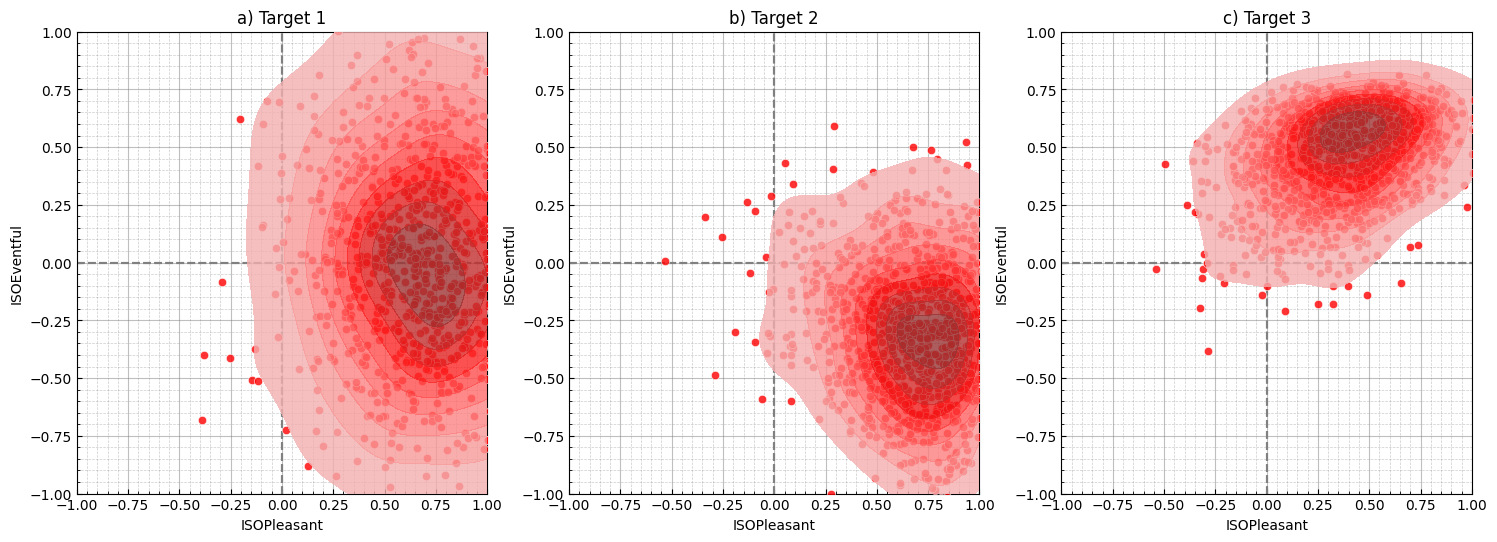
\includegraphics{Mitchell2024_JASA-SPI_files/figure-latex/notebooks-SingleIndex-Code-fig-tgts-output-1.png}

}

\caption{\label{fig-tgts}Example of defining and sampling from three
arbitrary bespoke targets.}

\end{figure}%

\textsubscript{Source:
\href{https://MitchellAcoustics.github.io/J2401_JASA_SSID-Single-Index/notebooks/SingleIndex-Code-preview.html\#cell-fig-tgts}{Exploring
defining single value indices - SPI }}

\subsection{Compare the target and test soundscape assessment
distributions}\label{compare-the-target-and-test-soundscape-assessment-distributions}

Central to the SPI framework is the concept of a distance metric, which
quantifies the deviation of a given soundscape from a desired target
soundscape. This distance metric serves as the basis for calculating the
SPI value, with smaller distances indicating a closer alignment between
the perceived soundscape and the target soundscape perception. The
distance between the test and target soundscape distributions is
calculated using a two-dimensional Kolmogorov-Smirnov distance
\(D_{BKS}\) \citep{Fasano1987multidimensional}. The KS distance is a
non-parametric metric of the equality of continuous distributions which
is sensitive to both the location and shape of the distributions
\citep{Chakravati1967Handbook}.

Essentially, we approach this as a problem of (dis)similarity between
soundscapes. The \(D_{BKS}\) distance metric is then proposed to assess
how similar any two given soundscapes distributions are within the
circumplex. Taken to the extreme, two perfectly matching distributions
in the soundscape circumplex would return a 100\% SPI value, while two
completely dissimilar distributions would return a 0\% SPI value. In
practical terms, for the former, this will never be achieved in real
world scenarios; for the latter, it is also difficult to estimate how
low the SPI value could actually go, and it should be considered that
the distance may happen in different directions within the circumplex
space. For instance, if a distribution for a vibrant soundscape was
taken as a reference, a compared soundscape distribution may exhibit low
SPI values for being located in the calm, OR monotonous, OR chaotic
regions of the model.

Using the data from one location in the ISD (Piazza San Marco) as the
test distribution, the \(D_{BKS}\) statistic is calculated for each of
the target distributions defined above, shown in Table~\ref{tbl-ks-test}
and \citet{fig}--targets.

\begin{longtable}[]{@{}
  >{\raggedright\arraybackslash}p{(\columnwidth - 4\tabcolsep) * \real{0.1528}}
  >{\raggedright\arraybackslash}p{(\columnwidth - 4\tabcolsep) * \real{0.0972}}
  >{\raggedright\arraybackslash}p{(\columnwidth - 4\tabcolsep) * \real{0.1944}}@{}}

\caption{\label{tbl-ks-test}Kolmogorov-Smirnov test comparing the
empirical test distribution (Piazza San Marco) against three soundscape
target distributions.}

\tabularnewline

\toprule\noalign{}
\begin{minipage}[b]{\linewidth}\raggedright
Target
\end{minipage} & \begin{minipage}[b]{\linewidth}\raggedright
D
\end{minipage} & \begin{minipage}[b]{\linewidth}\raggedright
\begin{verbatim}
      p
\end{verbatim}
\end{minipage} \\
\midrule\noalign{}
\endhead
\bottomrule\noalign{}
\endlastfoot
tgt\_1 & 0.66 & 6.94745e-25 \\
tgt\_2 & 0.83 & 8.96388e-39 \\
tgt\_3 & 0.28 & 8.96388e-39 \\

\end{longtable}

\textsubscript{Source:
\href{https://MitchellAcoustics.github.io/J2401_JASA_SSID-Single-Index/notebooks/SingleIndex-Code-preview.html\#cell-tbl-ks-test}{Exploring
defining single value indices - SPI }}

\subsection{Calculate the SPI score}\label{calculate-the-spi-score}

The final step is to convert \(D_{BKS}\) into a more interpretable form
to use as a comparison across soundscapes. Since the KS distance is a
measure of dissimilarity, we first subtract it from one to give a
measure of similarity between the test distribution and the target
distribution. This is then scaled to produce a score which ranges from 0
to 100, giving the final SPI formula:

\[
\text{SPI} = 100 * (1 - D_{BKS}\{\text{MSN}_{test}, \text{MSN}_{tgt}\})
\]

To show the usefulness of the test-target paradigm, we calculated the
SPIs for each of the three target distributions for all the locations
included in the ISD, as shown in Table~\ref{tbl-ex-spis}. Since each
location is now assigned an SPI, this makes it possible to effectively
produce three separate rankings of soundscape quality for these
locations, depending on which target is considered the goal.

\begin{longtable}[]{@{}
  >{\raggedleft\arraybackslash}p{(\columnwidth - 6\tabcolsep) * \real{0.1279}}
  >{\raggedright\arraybackslash}p{(\columnwidth - 6\tabcolsep) * \real{0.2907}}
  >{\raggedright\arraybackslash}p{(\columnwidth - 6\tabcolsep) * \real{0.2907}}
  >{\raggedright\arraybackslash}p{(\columnwidth - 6\tabcolsep) * \real{0.2907}}@{}}

\caption{\label{tbl-ex-spis}SPI scores and rankings for the soundscapes
of locations included in the International Soundscape Database (ISD).}

\tabularnewline

\toprule\noalign{}
\begin{minipage}[b]{\linewidth}\raggedleft
Ranking
\end{minipage} & \begin{minipage}[b]{\linewidth}\raggedright
\(SPI_1\) (pleasant)
\end{minipage} & \begin{minipage}[b]{\linewidth}\raggedright
\(SPI_2\) (calm)
\end{minipage} & \begin{minipage}[b]{\linewidth}\raggedright
\(SPI_3\) (vibrant)
\end{minipage} \\
\midrule\noalign{}
\endhead
\bottomrule\noalign{}
\endlastfoot
1 & 70 RegentsParkFields & 61 CampoPrincipe & 71 SanMarco \\
2 & 69 CarloV & 52 CarloV & 62 TateModern \\
3 & 65 RegentsParkJapan & 50 PlazaBibRambla & 60 StPaulsCross \\
4 & 62 CampoPrincipe & 49 RegentsParkFields & 58 Noorderplantsoen \\
5 & 61 PlazaBibRambla & 45 MarchmontGarden & 55 PancrasLock \\
6 & 61 RussellSq & 44 MonumentoGaribaldi & 54 TorringtonSq \\
7 & 61 MarchmontGarden & 40 RussellSq & 48 StPaulsRow \\
8 & 61 MonumentoGaribaldi & 38 RegentsParkJapan & 48 RussellSq \\
9 & 59 PancrasLock & 38 PancrasLock & 47 MiradorSanNicolas \\
10 & 53 StPaulsCross & 32 MiradorSanNicolas & 43 CamdenTown \\
11 & 49 TateModern & 30 TateModern & 40 CarloV \\
12 & 48 StPaulsRow & 30 StPaulsCross & 36 MonumentoGaribaldi \\
13 & 43 MiradorSanNicolas & 28 TorringtonSq & 34 MarchmontGarden \\
14 & 38 Noorderplantsoen & 28 StPaulsRow & 33 PlazaBibRambla \\
15 & 35 TorringtonSq & 17 SanMarco & 33 CampoPrincipe \\
16 & 33 SanMarco & 16 Noorderplantsoen & 32 EustonTap \\
17 & 21 CamdenTown & 15 CamdenTown & 27 RegentsParkFields \\
18 & 15 EustonTap & 13 EustonTap & 27 RegentsParkJapan \\

\end{longtable}

\textsubscript{Source:
\href{https://MitchellAcoustics.github.io/J2401_JASA_SSID-Single-Index/notebooks/SingleIndex-Code-preview.html\#cell-tbl-ex-spis}{Exploring
defining single value indices - SPI }}

\section{Expanding the SPI framework}\label{expanding-the-spi-framework}

Section~\ref{sec-method} has defined and demonstrated the foundational
methodology for calculating an SPI score. This included how to: define
and sample a target distribution; prepare the test and target
distributions for comparison using the KS distance metric; and convert
this into an SPI score. To expand this methodology into an applicable
framework, we define two distinct types of targets: bespoke targets and
reference targets, each serving a unique purpose in the index
development process.

\subsection{Bespoke Targets}\label{bespoke-targets}

Bespoke targets are essentially a direct application of the foundational
method described above. Bespoke targets are tailor-made for specific
projects, reflecting the desired soundscape perception for a particular
application. These targets can be defined by stakeholders, designers,
policymakers, or decision-makers based on their unique requirements,
objectives, and constraints. This flexibility allows the SPI for a
specific project to be tailored to the desire of the stakeholders for
how that specific soundscape should function. It can also provide a
consistent and quantifiable baseline for scenarios like a soundscape
design contest wherein a target is specified and provided to all
participants in the contest and the winning proposal is the design with
the highest SPI score when assessed against that target. Stakeholders
could use various methods to decide on a target, subject to the
requirements of their project or use case. For example, it could be
co-created with other stakeholders or space users, based on trying to
match the soundscape of a previous project, or entirely arbitrary.

\subsection{Reference Targets}\label{reference-targets}

In contrast to bespoke targets, reference targets represent generalized,
widely recognized soundscape archetypes which transcend specific
applications or projects. These archetypes serve as reference points and
enable comparisons across different domains and use cases. Essentially a
reference target is a target that has been \emph{empirically defined} to
encapsulate the ideal of a particular type of soundscape (e.g.~for a
park, for an urban square, for a particular group of users, etc.).

\subsubsection{Deriving a target based on a priori
rankings}\label{sec-targets}

Absent from the above methodology has been an exploration of how to
actually arrive at a target based on empirical evidence; i.e., not a
target specified \emph{ad hoc}, but rather an ``absolute'' target, based
on type of space, use case, or similar. While arbitrary targets make the
SPI framework incredibly flexible, able to score against an effectively
infinite set of design goals, often targets should have some sort of
systematic foundation, especially when defining a Reference Target. To
enable this approach, we therefore present one method of systematically
deriving a target distribution based on a given ranking of soundscape
quality. Just as one primary goal of the SPI framework is to enable
soundscape rankings to be produced from SPI scores, this method allows
for rankings which were arrived at separately to produce an optimised
SPI target.

The core challenge in developing a reference SPI target is determining
what constitutes an ``ideal'' soundscape perception distribution for a
given context. While we can directly specify MSN parameters to create
bespoke targets based on theoretical expectations or design goals,
developing empirically-grounded reference targets requires a more
systematic approach.

To enable this approach, we therefore present one method of
systematically deriving a target distribution based on a given ranking
of soundscape quality. The \emph{a priori} ranking serves as a bridge
between existing knowledge about soundscape quality and the mathematical
framework of the SPI. By starting with a ranking of soundscapes whose
relative quality has been assessed through some external measure, we can
use optimization techniques to derive MSN parameters that:

\begin{enumerate}
\def\labelenumi{\arabic{enumi}.}
\tightlist
\item
  When used as an SPI target, produce scores that result in the same
  ranking order
\item
  Generate high SPI scores for the highly-ranked soundscapes
\item
  Define a distribution in the circumplex space that captures the
  perceptual characteristics common to high-quality soundscapes in this
  context.
\end{enumerate}

This approach allows us to work backwards from known good (and poor)
examples to define what the target distribution should look like. For
instance, if we know that location A has a better soundscape than
location B for our purposes, the optimal target distribution should
result in location A receiving a higher SPI score than location B.

In this case study, we will examine a possible ranking from the ISD park
locations produced by the authors (shown in
Table~\ref{tbl-isd-ranking}).

\begin{longtable}[]{@{}cc@{}}
\caption{A pre-defined ranking of soundscape quality of the park
locations included in the International Soundscape Database (ISD). An
SPI target will be derived which aims to reproduce this same ranking
when applied to circumplex data from these
locations.}\label{tbl-isd-ranking}\tabularnewline
\toprule\noalign{}
Rank & Location \\
\midrule\noalign{}
\endfirsthead
\toprule\noalign{}
Rank & Location \\
\midrule\noalign{}
\endhead
\bottomrule\noalign{}
\endlastfoot
1 & RegentsParkJapan \\
2 & RegentsParkFields \\
3 & CampoPrincipe \\
4 & MonumentoGaribaldi \\
5 & RussellSq \\
6 & MiradorSanNicolas \\
7 & StPaulsCross \\
8 & Noorderplantsoen \\
\end{longtable}

Effectively, this is an optimisation task to determine the MSN
parameters which best achieve the above goals. Parameter optimisation
refers to the process of adjusting the parameters of a system, model, or
algorithm to achieve the best possible performance according to one or
more objectives. To set up the optimisation task, we first need to
express the parameter space and any constraints. Since our goal is to
identify an optimised soundscape target distribution, the parameters we
will search over are:

\begin{itemize}
\tightlist
\item
  \(\xi = (\xi_x, \xi_y)\), \(-1 \leq \xi \leq 1\)
\item
  \(\Omega = \begin{pmatrix} var(x) & cov(x, y) \\ cov(y, x) & var(y) \end{pmatrix}\)

  \begin{itemize}
  \tightlist
  \item
    \(0 \leq var() \leq 1\)
  \item
    \(-1 \leq cov() \leq 1\)
  \item
    \(\Omega\) must be symmetric and positive definite
  \end{itemize}
\item
  \(\alpha = (\alpha_x, \alpha_y)\), \(-5 \leq \alpha \leq 5\)
\end{itemize}

We then define the objective functions based on the two goals given
above. For each step in the algorithm with a given trial set of
parameters, a target distribution will be produced, the SPI for each
test location assessed according to the protocol described in
Section~\ref{sec-method}, and the resulting set of SPI scores and
ranking will be scored using the objective functions. Goal (1) is
assessed by calculating the Spearman rank correlation between the
\emph{a priori} ranking and the SPI ranking:

\[
f_1 = r_{s}(R(\text{prior}), R(\text{target}))
\]

Goal (2) is scored by calculating a weighted sum of the produced SPIs.
To prioritise a target which provides high SPI scores for highly ranked
soundscapes, we weight according to the ranking position:

\[
f_2 = \sum_{i=1}^m \frac{1}{\text{rank}_i} \cdot SPI_i
\]

where \(m\) is the number of included locations, \(SPI_i\) is the
calculated SPI score for the \(i\)-th location assessed against a trial
target, and \(\text{rank}_i\) is the calculated rank value of the
\(i\)-th location.

Through our testing, optimising only on the rank correlation regularly
produced targets which, while they did result in the desired ranking,
were in no way representative of the soundscapes in question. We
therefore aim to optimise for both a consistent soundscape ranking and
for a high SPI score for the top-ranked soundscapes. Optimising these
parameters with respect to multiple objectives ensures a more holistic
approach to system improvement, acknowledging the trade-offs and
interactions between different goals.

We apply the nondominated sorting genetic algorithm (NSGA-II)
\citep{Deb2002fast} to optimise our target distribution parameters.
NSGA-II is a popular and efficient multi-objective evolutionary
algorithm that is well-suited for problems with multiple, potentially
conflicting objectives.

The algorithm works as follows\footnote{Further technical details of the
  multi-objective optimisation procedure and the relevant code can be
  found in the Supplementary Material.}:

\begin{enumerate}
\def\labelenumi{\arabic{enumi}.}
\tightlist
\item
  Initialize a population of candidate solutions, each representing a
  set of target distribution parameters \((\xi, \Omega, \alpha)\).
\item
  Evaluate each candidate solution using the two objective functions
  defined above.
\item
  Perform non-dominated sorting to rank the solutions based on Pareto
  dominance.
\item
  Calculate crowding distance for each solution to maintain diversity in
  the population.
\item
  Select parent solutions using tournament selection based on
  non-domination rank and crowding distance.
\item
  Create offspring solutions using crossover and mutation operators,
  ensuring that the constraints on the parameters are maintained.
\item
  Combine parent and offspring populations and select the best solutions
  to form the next generation.
\item
  Repeat steps 2-7 for a specified number of generations or until a
  termination criterion is met.
\end{enumerate}

The NSGA-II algorithm is implemented using the Python library
\texttt{pymoo\ v0.6.1.3} \citep{pymoo}. The population size is set to
150, and the algorithm runs for 100 generations. In \texttt{pymoo}, each
objective function is supposed to be minimised, so when implementing the
algorithm and in the results, \(-f_1\) and \(-f_2\) are used. After
running the NSGA-II algorithm, we obtain a set of non-dominated
solutions representing the Pareto front, shown in
Figure~\ref{fig-pymoo-parks} (a). Each solution on the Pareto front
represents a trade-off between the two objectives: maximising the rank
correlation (\(f_1\)) and maximising the weighted sum of SPI scores
(\(f_2\)). The Pareto front allows us to visualise and analyse the range
of possible solutions, from those that prioritise ranking consistency to
those that emphasise high-SPI scores for top-ranked soundscapes.

\begin{figure}

\begin{minipage}{0.50\linewidth}

\centering{

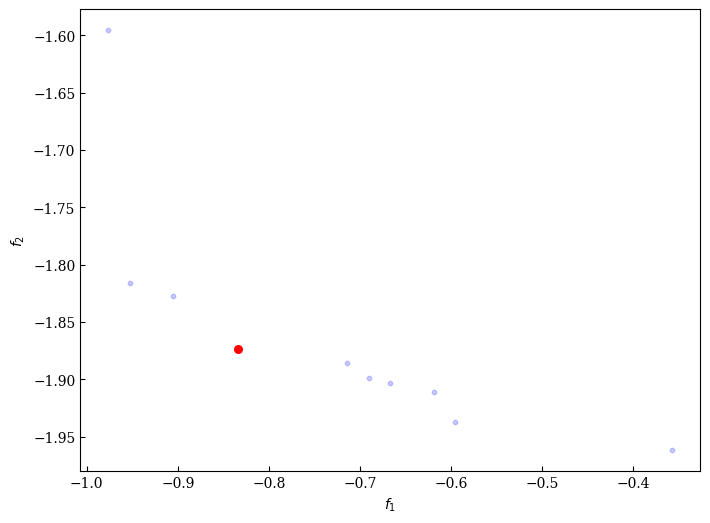
\includegraphics{Mitchell2024_JASA-SPI_files/figure-latex/notebooks-TargetOptimization-fig-pymoo-parks-output-1.png}

}

\subcaption{\label{fig-pymoo-parks-1}Multi-objective optimization Pareto
front. The selected solution is indicated in red.}

\end{minipage}%
%
\begin{minipage}{0.50\linewidth}

\centering{

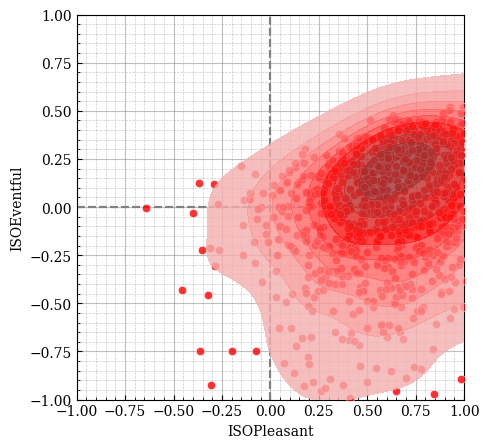
\includegraphics{Mitchell2024_JASA-SPI_files/figure-latex/notebooks-TargetOptimization-fig-pymoo-parks-output-2.png}

}

\subcaption{\label{fig-pymoo-parks-2}SCM distribution of the derived
target distribution.}

\end{minipage}%

\caption{\label{fig-pymoo-parks}NSGA-II optimization to learn the MSN
parameters which produce the Park ranking.}

\end{figure}%

\textsubscript{Source:
\href{https://MitchellAcoustics.github.io/J2401_JASA_SSID-Single-Index/notebooks/TargetOptimization-preview.html\#cell-fig-pymoo-parks}{Supplementary
Material for: Soundscape Perception Indices (SPI) }}

For this demonstration, we opt for the second method, selecting the
solution closest to the ideal point in the normalised objective space.
This approach provides a balance between ranking consistency and high
SPI scores for top-ranked soundscapes. Once the optimal solution is
selected, we can sample from the MSN distribution and plot the derived
target distribution, shown in Figure~\ref{fig-pymoo-parks}.

\[
\textup{tgt}_{\textup{park}} \sim  \left\{\begin{matrix}
    \xi&=&[0.694, 0.406] \\
    \Omega&=&\begin{bmatrix}
        0.157 & 0.040 \\ 
        0.040 & 0.255 
    \end{bmatrix} \\
    \alpha&=&[5.054, -37.671]
\end{matrix}\right.
\]

The resulting \(\text{tgt}_{\text{park}}\), with the MSN parameters
given above, exhibits some expected characteristics: it is almost
entirely pleasant, with a long uneventful tail into the calm quadrant,
but somewhat unexpectedly the mode is slightly vibrant. What should be
made clear about this demonstration is that we are not presenting this
as a reference target to be used in the future - this section is meant
as a demonstration of a method which can be used to derive a target from
an \emph{a priori} ranking. In this case, the \emph{a priori} ranking
was created by the authors from their experience of the locations in the
ISD. To truly be called an empirical reference target, the ranking would
need to be arrived at empirically, via some other metric (e.g.~health or
productivity ratings of the areas) or through an experiment such as
paired-choice comparisons.

It is these reference targets with an empirical backing which would
ideally form agreed upon standards and benchmarks in the field against
which new soundscapes would be compared. The best methods for
empirically determining the ideal soundscape distribution for a given
context will no doubt remain a topic of debate and development in the
coming years.

\section{Discussion}\label{sec-discussion}

The development of Bespoke and Reference context-dependent SPIs
represents a significant step towards enabling more comprehensive and
effective applications of the soundscape approach. By providing a
unified framework for defining these indices, the potential for
quantifying and comparing soundscape quality across diverse contexts and
applications is unlocked, while still ensuring that the
multi-dimensional and context-driven aspects of soundscape quality are
considered.

\subsection{Applications of the SPI
framework}\label{applications-of-the-spi-framework}

The proposed framework offers several key advantages. First, it
acknowledges the inherent context-dependent nature of soundscape
perception, allowing for the creation of indices tailored to specific
use cases or design goals through the use of bespoke targets. This
flexibility ensures that the resulting SPIs accurately capture the
desired soundscape perception for the given application, enabling
targeted interventions and optimisations.

Second, the inclusion of reference targets facilitates cross-comparisons
and benchmarking, enabling a common language and understanding of
soundscape quality across different domains. By calculating the distance
between a given soundscape and these widely recognized references,
stakeholders can identify areas for improvement and prioritize
interventions accordingly, aligning their efforts with collectively
recognized standards of desirable or undesirable soundscapes.

We expect that this would then expand into collections of SPI targets.
As an example, imagine trying to define a soundscape perception index
that could be applied across an entire city. A single index is
insufficient, because each type of place within the city (e.g.~parks,
plazas, residential areas) has different requirements for its
soundscape. Therefore, each place type would need its own soundscape
target.

In this example, these sets of targets would correspond to different
types of places within the city (e.g.~a single target for parks, a
target for plazas etc.). When applying this ``urban typology'' set of
targets, the soundscape of each location being assessed would be scored
against its relevant target (i.e how well does a specific park perform
in comparison to a reference park target). This results in a single
score for each location that can be compared against all other
locations, regardless of whether or not they are the same type of place,
allowing for different soundscapes to be compared on a common scale.
This system ensures that context (in this case, the typology of a space)
is brought into the assessment, allowing soundscapes to be scored
against the most appropriate target. Enabling these context dependent
assessments to be expressed on a common scale can facilitate additional
use cases such as soundscape mapping, which requires a single scale to
be applied across an entire city.

This set of targets made up of e.g.~parks, plazas etc. is just one
example of an application of reference SPIs. Other examples could
include a demographics SPI, where different targets are set for
respondents from different demographic groups, or a ``use case'' SPI
with different targets set for different intended purposes of spaces
(e.g.~recreation, restoration, socialising). We encourage users of the
SPI to define both their own single reference targets that can be added
these suites of targets for use by others, and their own new sets of
reference.

\citet{Kogan2018Green}, Fig.6, in fact displays a startlingly similar
concept, showing the locations of the three categories of traffic noise
dominance (`traffic noise', `balanced', and `natural') plotted in the
circumplex perceptual model. It can be clearly seen in this plot that
the GSI categories create their own clusters within the circumplex.

Although it is expected that the target distribution would usually
represent the ideal or goal soundscape perception, it is also possible
to define target distributions that represent undesirable or suboptimal
soundscape perceptions. For instance, in a soundscape mapping context,
it may be beneficial to map and identify chaotic soundscapes across a
city in order to better target areas for soundscape interventions. In
this case, the target distribution would be set in the chaotic quadrant
and a higher SPI would indicate a closer alignment with the target
distribution. This flexibility allows the SPI to be applied to a wide
range of contexts and applications, enabling the quantification and
comparison of soundscape quality across diverse scenarios.

\subsection{Connecting with soundscape
data}\label{connecting-with-soundscape-data}

Unlike previous soundscape indices (see
Section~\ref{sec-existing-soundscape-indices}), SPI does not include any
direct connection to soundscape indicators such as the sound level,
spectral content, etc. Its basis in perceptual descriptor data effective
allows the analysis and quantification of soundscape information to be
modularised, separating the task of calculating a single index from the
complex task of predicting soundscape perception from objective data.
The modularisation of soundscape data analysis allows the entire
pipeline from environmental data collection through to soundscape index
scoring to remain flexible. Following the soundscape engineering
paradigm laid out in \citet{Mitchell2023conceptual}, the connection
between soundscape indicators, through descriptors, to indices can be
made by predictive soundscape models. These models are trained on
increasingly large scale datasets and generally designed to predict
soundscape descriptors, including the SCM attributes
\citep[@Hou2024Soundscape]{Ooi2022Probably}. With the complex and
multidimensional nature of soundscape perception and with the rapid
progression in machine learning techniques and applications, an index
framework should be able to integrate new and improved models. By
separating the prediction of perceptual descriptors based on objective
metrics from the calculation of the single value index itself, the SPI
framework allows for these predictive models and for the creation of new
indices to advance independently.

\subsection{Comparison with existing soundscape
indices}\label{comparison-with-existing-soundscape-indices}

The SPI framework represents a unique approach to soundscape assessment,
building upon and differentiating itself from previous indices in
several key ways. Firstly, the SPI framework is fundamentally
perception-focused. By referring to the ``Soundscape Perception Index'',
we aim to highlight the unique and perception-focussed nature of this
index framework. The SPI core method operates entirely within the
perception data space, with no direct reference to acoustic or other
indicators. Perceptual data (or predicted perceptual data) are the only
operant factors of the SPI method. The aim of SPI is to combine
multidimensional perception data and context (including design goals)
into a single metric.

The SPI framework shares this important characteristic with indices like
the Soundscape Diversity Index (SDI) \citep{Liu2014Effects} and the
Harmonious Degree of Sound Sources (SHD) \citep{Guo2023Harmonious} in
that they all prioritize perception as the primary input for assessment.
Both SDI and SHD, however, focus on the perception of sound sources that
can be observed in an acoustic environment, and their relationships.
While these indices offer valuable insights into specific aspects of
soundscape perception, they are somewhat limited in their scope and
adaptability. The SPI framework builds upon these efforts by
incorporating the full dimensionality of the soundscape circumplex model
and allowing for context-sensitive assessments through bespoke and
reference targets. This approach enables the SPI to address a wider
range of soundscape evaluation needs while maintaining the crucial focus
on perceptual data that distinguishes these methods from purely acoustic
measurements.

Furthermore, the SPI framework is designed to be generalisable,
extensible, and adaptable. Unlike previous indices that often represent
a single target in a particular context, the SPI framework allows for
scoring soundscapes against any goal defined by the user. This
flexibility makes it applicable across a wide range of contexts and
design objectives, from urban planning and acoustic design to research
and policy development.

\subsection{Considerations and future work}\label{limitations}

Several considerations should be noted when defining an SPI target.
First, the target distribution should be representative of the desired
soundscape perception for the given application. This requires a clear
understanding of the context, objectives, and constraints of the
project, as well as the preferences and expectations of stakeholders and
end-users. Second, the temporal and spatial scales of the target
distribution should align with the soundscape assessment being
conducted. What constitutes the actual spatial bounds of `a soundscape',
or indeed of `a place', is a complex question which will depend on the
context of the assessment. For example, a park soundscape may be defined
by the boundaries of the park itself, or it may extend to include the
surrounding urban environment or be restricted to a certain distance
from a feature of interest in the park\footnote{For instance, the SSID
  Protocol, which produced the data used in this paper, attempted to
  address this by considering its spatial bounds for what constitutes
  one location to be ``an `environmental unit' wherein the environmental
  factors are consistent and is typically perceived to constitute a
  single distinct area'', noting that ``the exact dimensions and
  delineation of the environmental unit will vary depending on the
  characteristics of the space'' \citep{Mitchell2020Soundscape}}. The
temporal scale of the assessment is also important, as soundscape
quality can vary throughout the day and across different seasons.
Increasing the spatial bounds of what is considered the soundscape under
examination (e.g.~a single position vs a 25\(m^2\) area vs an entire
park) or extending the temporal scale will almost certainly result in a
distribution with a larger variance. What scales are appropriate for a
given assessment will depend on the context and objectives of the
project, but they should be considered when defining the target
distribution. Applying a target distribution that is too broad or too
narrow for the context of the assessment may result in inaccurate or
misleading SPI scores. As the circumplex distribution first described in
\citet{Mitchell2022How} and further formalised here develops, we are
hopeful that a better understanding of the relationship between temporal
and spatial scales and the parameters of the distribution will emerge
and will contribute to an increased understanding of what constitutes
`the soundscape of a place' and how this should be reflected in its
ideal perception distribution.

Various other distance metrics were considered when developing the SPI
method. The simplest method is to define a single point target, rather
than a target distribution, and calculate a normalized mean Euclidean
distance between points in the test distribution and the target point.
While this is conceptually simple and requires defining only a single
coordinate point as a target, rather than the MSN parameters described
in Section~\ref{sec-circumplex-distribution}, the shape and spread of a
soundscape distribution is itself an important factor in describing the
collective perception of a soundscape and would not be captured by this
method \citep{Mitchell2022How}.

An additional method which was considered, was to consider a target as
an ellipse (or, indeed any other shape) drawn in the circumplex space
(similar to the simplified median decile curves proposed in
\citet{Mitchell2022How}). An SPI score would then be calculated based on
the percentage of responses which fall within the space defined by the
ellipse. Again, this is conceptually quite simple and defining the
ellipse targets is straightforward. However, this method has an
important flaw - it is easy to artificially inflate or deflate the
scores merely by changing the area of the ellipse. The larger the
ellipse, the higher all SPI scores will be, regardless of whether the
sample distribution is wide or narrow. This would also limit
cross-comparability between targets. As can be seen in
Table~\ref{tbl-ex-spis}, defining a target distribution with a larger
spread (i.e.~\(\text{tgt}_1\)) does not automatically result in higher
SPI scores across the board as it would with the ellipse target method.
By defining the SPI as a true target-test distribution comparison we
ensure that the SPI always accurately reflects the similarity between
the perception of a soundscape and its target, both in terms of its
location in the circumplex and the shape of the data.

As noted in Section~\ref{sec-targets}, although a methodology for
deriving targets is presented, the \emph{a priori} ranking we use for
the demonstration was not itself arrived at empirically. Hence the park
target cannot be considered a true reference target. A key piece of
future work is to use experimental methods such as paired-choice
comparisons to arrive at a well-defined ranking which can then produce a
true reference target.

\section{Conclusion}\label{conclusion}

The ERC-funded Soundscape Indices (SSID) project was started mostly with
the ambition to derive soundscape indices that could serve as
numerical/quantifiable tools \citep{Kang2019Towards}, to better inform
urban sound planning and design decisions. Any soundscape researcher
having ever made an attempt at defining ``the'' soundscape quality index
will know what a challenging, even impossible, task this is. Some may
even argue that trying to reduce soundscape quality to a single-value
quantity, and deriving any soundscape index, could be what philosophers
would call a \emph{contradictio in adjecto}, as the soundscape approach
intrinsically advocates for a multi-dimensional characterization of the
acoustic environments that we experience in our lives. For these
reasons, we felt that it was necessary to take a step back and create
instead a framework tailored for the field specifically that could
easily be adapted to different contexts and capture the multi-faceted
aspects of the soundscape of a place.

The proposed framework addresses the existing gap in quantifying
multi-dimensional soundscape perception, facilitating a broader
application of the soundscape approach in areas such as urban planning,
environmental management, acoustic design, and policy development.
Through the creation of bespoke indices tailored to specific design
goals and the utilization of reference targets for benchmarking, this
framework empowers stakeholders and decision-makers to make informed
choices and prioritize soundscape improvements aligned with their unique
objectives and constraints.

Furthermore, the grounding of the SPI framework in the soundscape
circumplex model ensures a robust theoretical foundation, capturing the
multi-dimensional nature of soundscape perception. The use of a distance
metric enables quantitative assessments and comparisons, fostering a
common language and understanding of soundscape quality across different
domains. This shared understanding facilitates knowledge exchange,
collaborative efforts, and the development of best practices within the
field. As the SPI framework continues to be explored and refined, future
research should focus on validating and expanding the range of reference
targets, as well as investigating the potential for incorporating
additional dimensions and factors that influence soundscape perception.
The integration of emerging technologies (such as virtual, mixed, and
augmented reality) may also provide new avenues for immersive soundscape
evaluation and index development. Additionally, the application of the
framework in diverse real-world scenarios, ranging from urban planning
and environmental management to acoustic design and policy development,
will provide valuable insights and contribute to the ongoing refinement
and adaptation of the SPI framework.

In many ways, the proposed SPI framework is not so conceptually
different from the whole idea of decibel-based set of indicators that
the Soundscape Indices (SSID) project itself is trying to ``overcome''.
There is no such thing as a single noise indicator (\emph{L}) to
univocally describe sound levels in all circumstances; rather, different
noise indicators are defined for different scenarios and temporal or
spectral requirements (e.g., \(L_{den}\), \(L_{Aeq, T}\), etc.), based
on testing needs. The decibel (dB) is the unit for all of them, but
A-weighted equivalent sound levels for a one-hour interval cannot be
directly compared with whole-day indicators with penalties. We are
trying to achieve the same with the SPI to provide a way of defining
different indices for different contexts, while maintaining a consistent
framework.

Ultimately, for the SPI approach to succeed, collaboration with
stakeholders, end-users, and experts from various domains will be
crucial in ensuring the framework's relevance and applicability across a
wide range of contexts.

\section*{Acknowledgements}\label{acknowledgements}
\addcontentsline{toc}{section}{Acknowledgements}

This project has received funding from the European Research Council
(ERC) under the European Union's Horizon 2020 research and innovation
program (Grant No.~740696, project title Soundscape Indices - SSID).
More information and related publications can be found at the CORDIS
webpage of the project\footnote{See
  \url{https://cordis.europa.eu/project/id/740696/factsheet} (Last
  viewed 2024-05-28).}

\section*{Data and Code Availability}\label{data-and-code-availability}
\addcontentsline{toc}{section}{Data and Code Availability}

The data used in this paper are drawn from the publicly available
International Soundscape Database (ISD v1.0.1-alpha.1)
\citet{Mitchell2024International} available on Zenodo\footnote{See
  \url{https://doi.org/10.5281/zenodo.10672568}}. The code to recreate
the figures in this paper can be found on this paper's Github
page\footnote{See
  \url{https://github.com/MitchellAcoustics/J2401_JASA_SSID-Single-Index}}.

\section*{Author contributions}\label{author-contributions}
\addcontentsline{toc}{section}{Author contributions}

\textbf{AM}: Conceptualization, Methodology, Software, Writing-Original
Draft, Writing-Review \& Editing, Visualization. \textbf{FA}:
Conceptualization, Methodology, Writing-Review \& Editing. \textbf{TO}:
Conceptualization, Writing-Review \& Editing. \textbf{JK}:
Conceptualization, Supervision, Funding acquisition.


\renewcommand\refname{References}
  \bibliography{FellowshipRefs2.bib}



\end{document}
